\documentclass[12pt]{article}
\usepackage[utf8]{inputenc}
\pagenumbering{arabic}
\usepackage{graphicx}
\usepackage{amstext}
\usepackage[usenames, dvipsnames]{color}
\usepackage{array}
\usepackage{float}
\usepackage{enumitem}
\usepackage[top=1.5in]{geometry}
\usepackage{subcaption}
\graphicspath{ {images/} }

\begin{document}

\begin{titlepage}
    \begin{center}
    \begin{figure}
        \centering
        
\includegraphics[scale=0.2]{logoPolimi.png}
        \vspace{1.5cm}
    \end{figure}

    \Huge\textbf{Software Engineering 2 Project - TrackMe}
    \rule{12cm}{0.5pt}
    \Huge\textbf{Design Document - V1.0}
    \vspace{1mm}
    \newline
    \today
    \end{center}
    
    \vspace{3cm}
    
    \begin{flushleft}
        \LARGE\textbf{Authors: }
        \newline\newline
        \Large\texttt{}{Michiel Janssen \\ Erbol Kasenov \\ Lorenzo Casalini}
    \end{flushleft}
\end{titlepage}

\newpage
  \tableofcontents
\newpage
\section{Introduction}

\subsection{Purpose}
The main purpose of the Software Design Document (or just Design Document) is to provide a more technical and detailed description than the RASD about the TrackMe application system. This document describes how TrackMe is designed and planned, identifying its main components and the interfaces between them. It also guides the software development team and other interested parties through the architecture of the software project, stating what has to be implemented and how to do it.
\vspace{3mm}
\newline 
More precisely, the document presents:
\begin{itemize}
    \item Overview of the high level architecture
    \item The main components and their interfaces provided one for another
    \item The Runtime behavior
    \item The design patterns
    \item The algorithm design of the most critical parts of the application
    \item Implementation plan
    \item Integration plan
    \item Testing plan
\end{itemize}
The purpose of this document is to provide an overall guidance to the architecture of the software product.



\subsection{Scope}
TrackMe is a company that wants to develop a software-based service allowing third parties to monitor the location and health status of individuals. The main service, Data4Help, supports the registration of individuals (of any age) and third parties. Upon registration the individual agrees that TrackMe acquires their data. This data can be obtained from smartwatches or similar devices. After registration a third party can request the following things:
\begin{itemize}
\item Access the data of a specific individual by entering a unique number or code. TrackMe passes the request to the specific individual who can accept or refuse the data acquisition.
\item Access anonymized data of groups of individuals given by a specific constraint e.g.: every individual older than 30 years, every individual that is male or female, etc. These requests are handled and approved by TrackMe if and only if TrackMe can guarantee that they are able to properly anonymize the requested data.
\end{itemize}
As soon as a data request is approved, TrackMe makes the previously saved data available to the third party. The service also allows a third party to subscribe to new data and listen to new data as soon as they are produced. With the data acquired through Data4Help, it will be also possible to offer two other services based on the retrieved data. The first service is a personalized and non-intrusive SOS service, called AutomatedSOS, to help elderly people. This service monitors the health status of subscribed customers and sends an ambulance to this specific customer if some parameters are below a certain threshold. The reaction time should be less than 5 seconds from the time the parameters are below the certain threshold.
The second service, called Track4Run, allows organizers to define a path for a run, participants to enroll to a certain run and spectators to see the position of all current running participants on a map.


\subsection{Definitions, Acronyms, Abbreviations}

\subsubsection{Definitions}

\begin{itemize}
\item \textit{Visitor}: A person who uses TrackMe for the first time, and is not yet registered. This can be an individual or a third party. After a successful registration process the person becomes an individual and is now able to use TrackMe services.
\item \textit{Individual}: A registered person who uses TrackMe for monitoring his location and health status.
\item \textit{Third party}: A registered organization that wants to access the location and health status of specific individual by giving a social security number of that individual.
\item \textit{System}: defines the overall set of software components that implement the required functionality.
\end{itemize}
\newpage 
\subsubsection{Acronyms}

\begin{itemize}
    \item \textit{API}: Application Programming Interfaces
    \item \textit{RASD:} Requirements Analysis and Specifications Document
    \item \textit{DD}: Design Document
    \item \textit{DB}: Database
    \item \textit{DBMS}: Database Management System
    \item \textit{ER}: Entity Relationship Model
    \item \textit{SQL}: Structured Query Language
    \item \textit{UX Diagram}: User Experience Diagram
    \item \textit{JSON:} JavaScript Object Notation
    \item \textit{REST:} Representational State Transfer
     
\end{itemize}
\subsubsection{Abbreviations}
\textit{Gn}: Goal defined with index n.\newline
\textit{Rn}: Functional Requirement defined with index n.
\subsection{Revision History}
\textbf{Version 1.0:} Initial Release

\subsection{Reference Documents}
\begin{itemize}
    \item RASD V1.0 produced before
    \item Assignment document: Mandatory Project Assignment AY 2018-2019.pdf
    \item Design Patterns by Jason McDonald (dzone.com/refcardz/design-patterns)
\end{itemize}

\newpage
\subsection{Document Structure}
Other than this introductory chapter, this DD is organized in seven more chapters.
Chapter two is meant to \textbf{provide different types of views over the system:}
\begin{itemize}
     \item High level components and their interaction : this sections gives a global view of the components
     of the application and how they communicate
     \item Component view : this sections gives a more detailed view of the
     components of the applications

    \item  Deploying view : this section shows the components that must be
    deployed to have the application running correctly.

    \item  Runtime view : sequence diagrams are represented in this section to
    show the course of the different tasks of our application
    \item Component interfaces : the interfaces between the components are
    presented in this section

    \item Selected architectural styles and patterns : this section explain the
    architectural choices taken during the creation of the application


    \item Other design decisions
\end{itemize}

\noindent 
In the third chapter the most \textbf{relevant algorithms} are analyzed and discussed with the appropriate
detail and depth, in order to describe the way the system’s most critical operations are driven and executed
. Pseudo code is used for the algorithms in order to hide unnecessary implementation details.
The fourth chapter deals with the \textbf{user interface design}. This chapter mainly refers to the mockups 
provided in the RASD, but it will also include some details on the user interaction with the UI, illustrated
by a UX Diagram.
The fifth chapter explains how the \textbf{requirements defined in the RASD are fulfilled by the design 
decisions} that were taken, and how these \textbf{requirements map} to the design elements and decisions 
defined in the DD.
In the sixth chapter, a \textbf{implementation, integration and test plan} is provided, defining the 
order in which the different subcomponents of the system will be implemented, the 
order in which they will be integrated and how this integration will be tested alongside with the
development of the system.
In the seventh chapter the \textbf{effort spent by each of the group members} is described by specifying the
number of hours each member of the group worked on the development of this document and, on the final
chapter, \textbf{the tools we used to develop this DD are specified.}  


\section{Architectural design}

\subsection{Overview: High-level components and their interaction}
In the following paragraphs a general overview of how the system is architected will be presented,
especially focused on the different logically separated layers. As described on the RASD, TrackMe is
supposed to be fully scalable and portable, so a layered architecture is the one that best fits these
requirements. Given that the system only provides an Application interface, there’s no need for a fourth
layer isolating the web server from the application server.
With this in mind, the system will have a three-layer architecture, organized as shown below:

\begin{figure}[H]
\centering
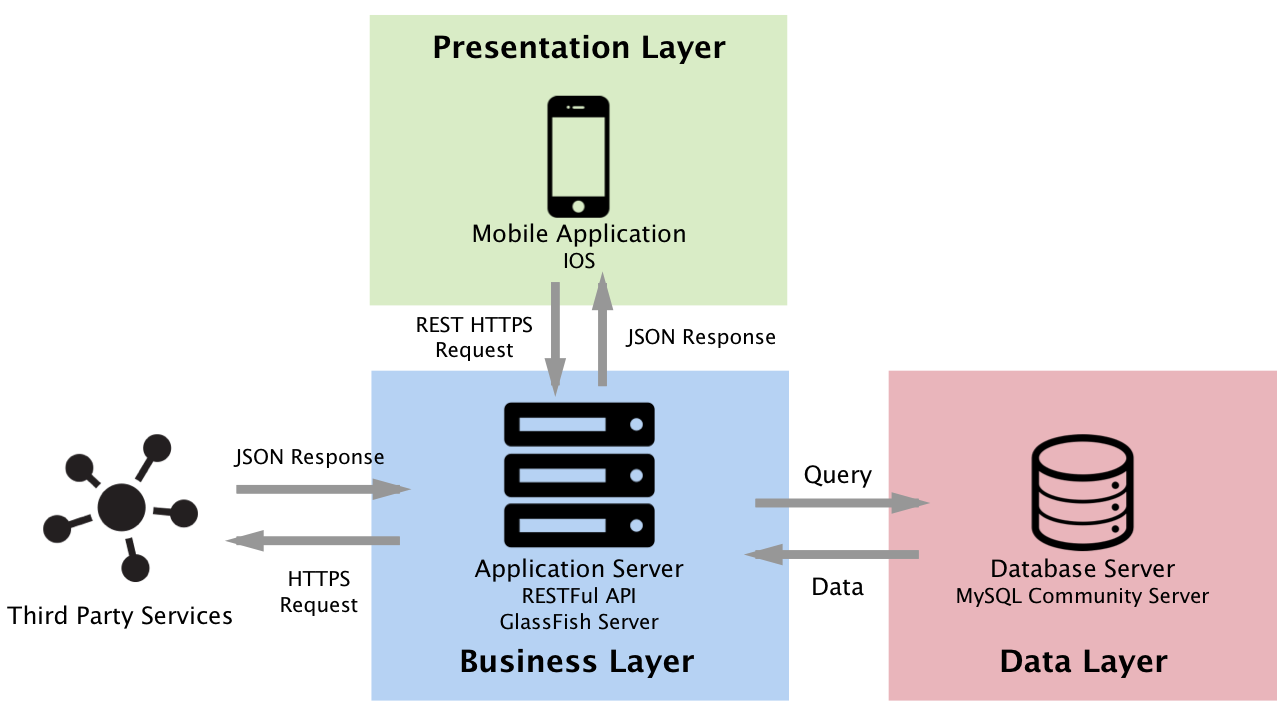
\includegraphics[scale=0.6]{highLevelView.png}
\label{fig:highLevelView}
\caption{High Level View of the system's architecture.}
\end{figure}
\noindent 
\begin{itemize}
    \item \textbf{Presentation Layer:} is the most external layer of the system, and is respon- sible for handling all GUI communication and logic. This layer does not handle data or process business rules, but it forwards all the requests to the layers bellow and translates the system operations results of these requests to something that users can understand. It is the only layer of the system that users can access directly and interact with.
    \newpage
    \item \textbf{Business Layer:} implements all core functionality of the system. It's in this layer that the application logic and business rules are implemented, in particular, all the operations related to a individual or third party account and health data creation are performed by components of this layer. This layer interacts with the APIs exposed by the Data Layer in order to store and retrieve data. The business layer also depends on some third party systems and the external services they provide (specifically for the implementation of the health data creation we rely on external devices to monitor data). These external services are directly invoked by some of the classes of the Business Layer using a public API provided by those.
    \item \textbf{Data Layer:} is the lowest layer of the architecture and includes the data persistence mechanisms responsible for data storage and management. It also provides an API to the Business Layer that exposes methods of managing the stored data without creating dependencies on the data storage mechanisms, promoting the encapsulation of the persistence mechanisms and avoiding data exposition.
    \item \textbf{Third Parties:} Even though they don't belong to any particular layer, these services are illustrated in the figure above in order to highlight that the interaction with the hird parties will happen at the level of the Business Layer.
\end{itemize}

\subsection{Component view}
The main function of this section is to present a more detailed description of the components that must be
developed as part of TrackMe. In the following diagram, we can see the component view of the system (the
more complex components will be analyzed in further detail).

\begin{figure}[H]
\centering
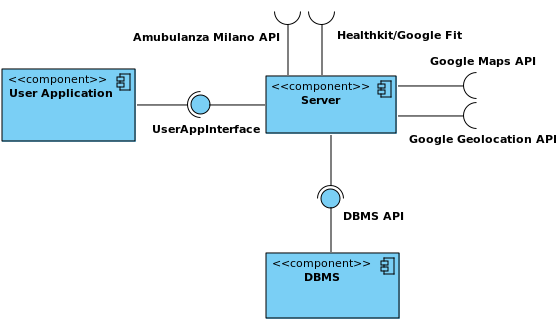
\includegraphics[scale=0.5]{ComponentDiagram1.png}
\label{fig:ComponentDiagram1}
\caption{Component Diagram of the system.}
\end{figure}
\newpage
\noindent 
The \textbf{User Application} is the component responsible for providing the user interfaces that allow
the user to interact with the system and all of its functionality. Since a thin-client architecture is being
used to implement a client/server architecture, the bulk of the data processing occurs on the server.
Given this, the User Application component will act as a simple "terminal" to send requests to the server,
being therefore quite simple and not needed to go into further detail.
\newline \noindent The \textbf{Server} is the main component of the system, responsible for the data
processing in order to provide all of the system’s functionality. Given its complexity, it will be analyzed
in further detail later in this section.
\newline \noindent The \textbf{DBMS} is the component responsible for storing and retrieving data in a 
persistent and reliable way. Instead of implementing this component from scratch, a commercial solution 
shall be used (MySQL for example).

\subsubsection{Server detailed analysis}

\vspace{3mm}
\noindent Being the most complex component of the system, it is useful to analyze in detail the Server's 
constitution. As mentioned previously, this component is primarily responsible for all operations related 
to the system's functionality. More specifically, this component is divided into six sub-components, each 
related to a different kind of functionality and operations (diagram can be found in figure ~\ref{fig:serverComponentView}):

\begin{itemize}
    \item The \textbf{Router} sub-component receives the requests from the User Application and forwards (routes) them to the corresponding controller.
    \item The \textbf{Health Data Controller} sub-component is the one who performs all the necessary
          operations that allow the user to collect all his health data acquired and made through external devices. This module is the one with more external interfaces since it needs to gather all health data from individuals and their location from the external devices. This sub-component is also responsible to communicate with the Ambulanza Milano API, so when a certain parameter is below a certain value the system can immediately ask to send the closest ambulance to the individual in danger. 
    \item The \textbf{Account Controller} sub-component implements all the methods for inserting or updating information about the users. More specifically, it allows the creation of new users (registration of visitors) and login of already existing users.
    \item The \textbf{Run Controller} sub-component implements all the methods so that every user can organize a path for a run and every individual can participate in a run or spectate runners. It uses information from the Health Data Controller and Account Controller to fulfill this requirements.

    \item The \textbf{Data Access Controller} sub-component (and all of its sub-components) manages the behavior and data of the application domain and responds to requests or instructions by the respective controller.
    \item The \textbf{Data Mappers} sub-component is a layer of software which separates the model from the database and acts as a "middle-man", the backend, for the interactions between these two.
\end{itemize}
\subsubsection{Database detailed analysis}
The following ER provides a graphical representation of the conceptual model of the database.
\vspace{20mm}

\begin{figure}[H]
\centering
\centerline{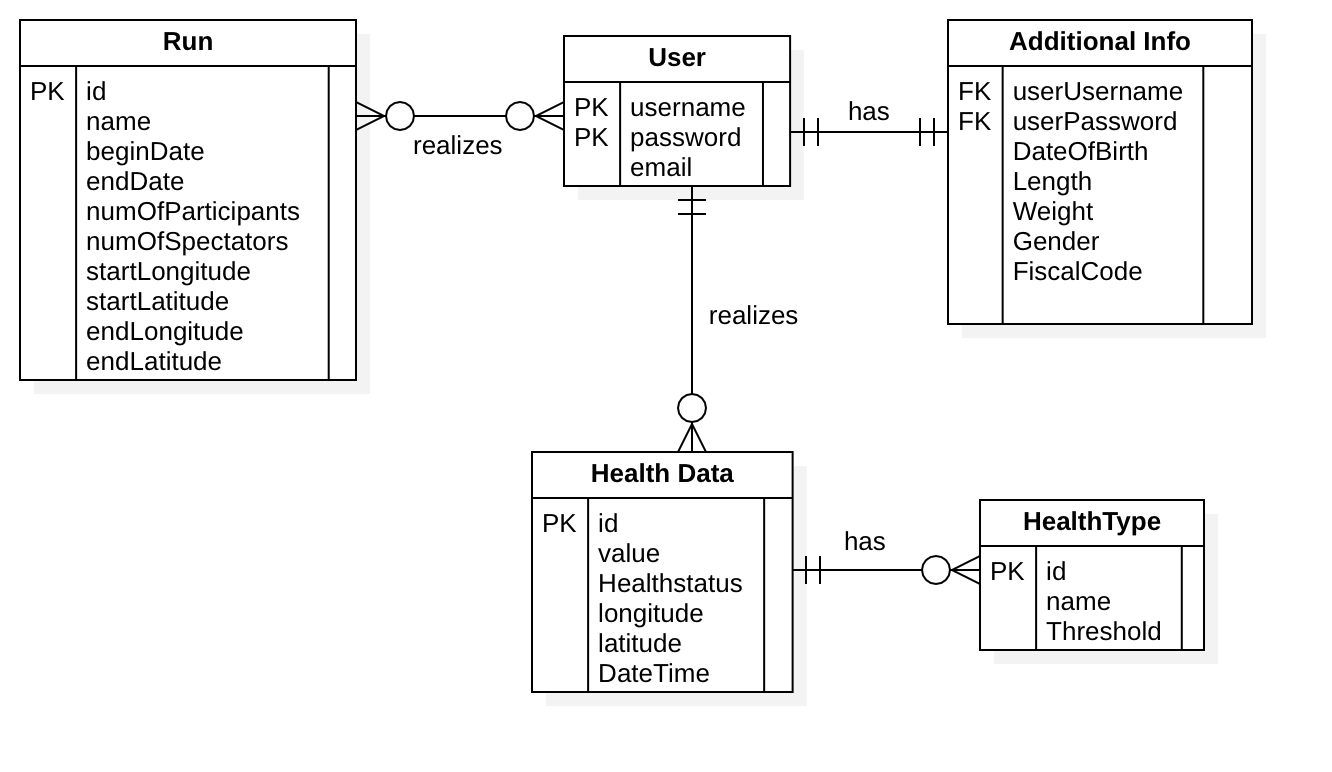
\includegraphics[scale=0.4]{databaseTrackMe.png}}
\caption{Database ER.}
\label{fig:databaseTrackMe}
\end{figure}



\begin{figure}[H]
\centering
\centerline{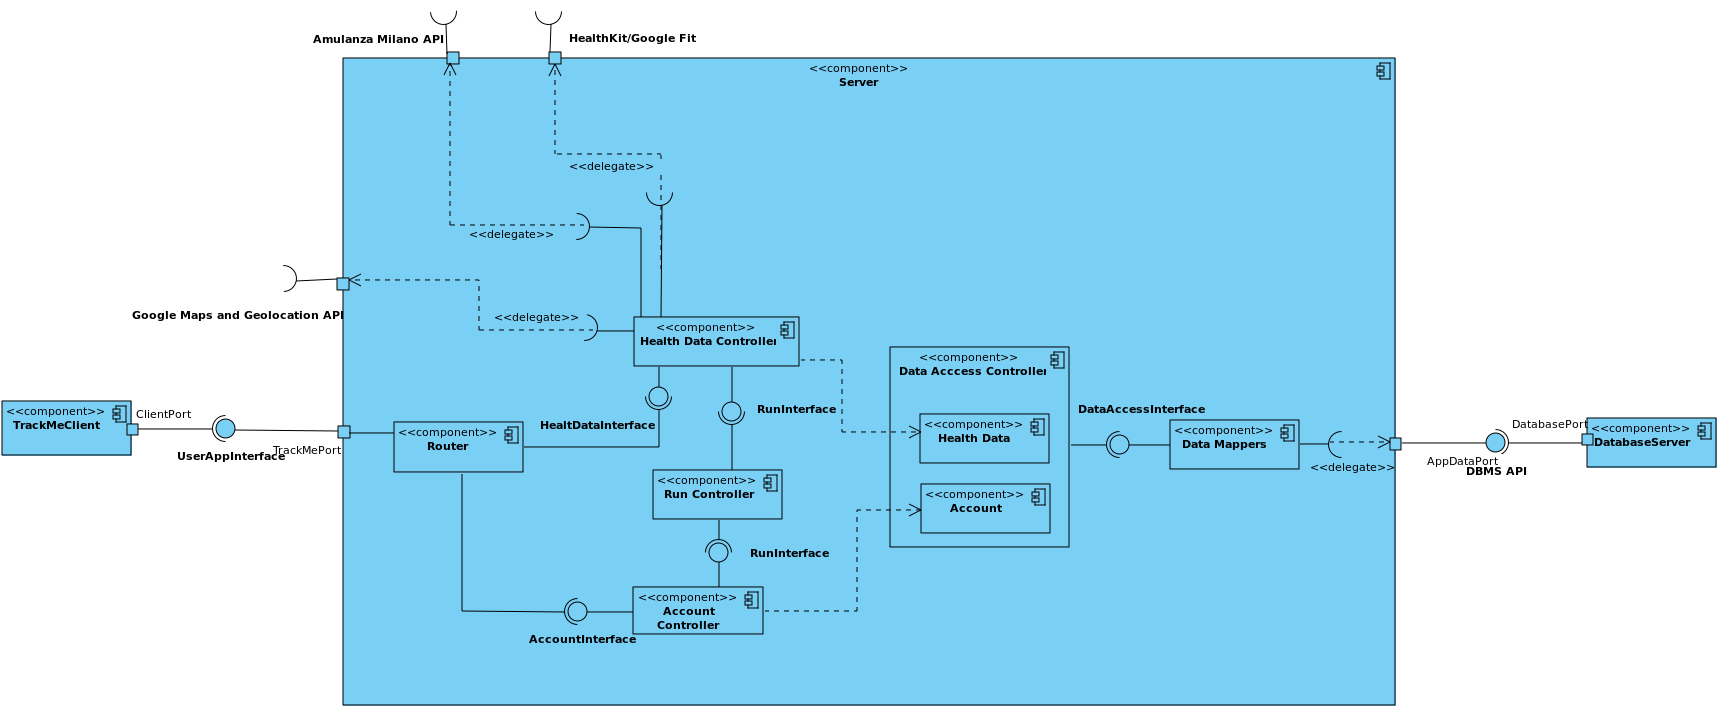
\includegraphics[scale=0.33, angle=-90,origin=c]{serverComponentView.png}}
\caption{View of Server Component in detail.}
\label{fig:serverComponentView}
\end{figure}


\subsection{Deployment view}
The main purpose of this section is to show how the software components described above are going to be 
deployed in the system's hardware infrastructures. This characteristic makes the developer's task easier 
since the mapping between software and hardware becomes explicit. The deployment diagram in figure ~\ref{fig:DeploymentView} shows the architecture of the system as deployment (distribution) of software artifacts
to deployment targets. TrackMe requires deployment of software on the following nodes:
\begin{enumerate}
    \item \textbf{User Application:} this is the application (TrackMe) that will be used by the user. The user will be able to get information from the main TrackMe server.
    \item \textbf{TrackMe server:} the main logic of the application will be deployed here. This server will communicate with all the other nodes. It will gather information from the external services (API's), manage user accounts and saved health data from the Database server and take requests and send back responses to the user.
    \item \textbf{Database server:} it will store all the persistent data for the users such as usernames and passwords, as well as their health data and data about the organization of runs.
    \item \textbf{External server:} it will only provide services to enrich the application. For example, Google Maps/Geolocation is used to locate an individual, HealthKit/Google Fit is used to track the health of an individual, etc.
     
\end{enumerate}


\begin{figure}[H]
\centering
\centerline{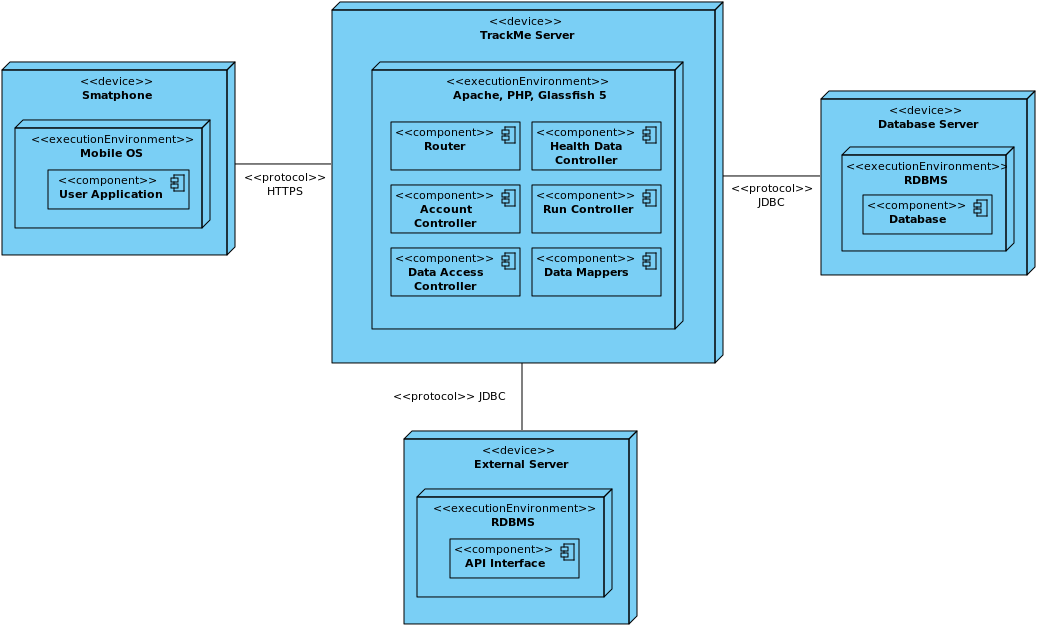
\includegraphics[scale=0.45]{DeploymentView.png}}
\caption{Deployment View of the system.}
\label{fig:DeploymentView}
\end{figure}

\subsection{Runtime view}
The following diagrams are intended to describe the interactions between the main system components when 
performing a sample amount of functionality. These diagrams are still a high-level view of the system, 
since the function names or even the functions themselves may change during the development process.

\begin{itemize}
    \item \textbf{Section 2.4.1:} in this sequence, the process of logging in a user is shown. The user fills in his credentials and passes it to the user application which checks if the provided data is valid. The router forwards the validity request to the DBMS to check if a match for the given username and password is found in the DB. If and only if the filled in data is valid (correct credentials) the user application displays a success. The result of this success is that the user is now successfully logged in and can use the TrackMe application. If no success has occurred the user application displays an error.
    \newpage 
    \item \textbf{Section 2.4.2:} in this sequence, the process of creating new health data for a user is shown. The component mainly used for this operation is the Health Data Controller. It's the user application (and not the user himself) who creates this health data. The user is not the one who is responsible for making the health data, he doesn't need to push on a button to retrieve new health data. The first time a user uses TrackMe, the user gives permission to TrackMe to track his health and further retrieving of available data is done automatically in the background by the user application. First the Health Data Controller retrieves specific data from HealthKit or Google Fit by entering the HealthDataDetails (this is usually a username). After retrieving the health data from the user, the Health Data Controller internally checks the healthstatus of the user. If and only if the threshold of a certain parameter, defined for each type health data, is violated (person is in danger) the system communicates with the Ambulanza Milano API and they will send an ambulance to the person in question. After that we try to make the health data. Only is the health data is makeable (health data won't be makeable if e.g.: you want to monitor the blood pressure of a user but this user isn't using a external device to measure the blood pressure. Therefore we can't retrieve this data and it's not makeable) it willed be placed inside the Health Data Controller health data queue. This queue is then uploaded to the database to store health data for each user. If nothing goes wrong we have successfully made new health data, otherwise an error will occur in the background stating that something went wrong when uploading data to the database. Last but not least if health data is not makeable there will also occur an error in the background of the user application.
    
    
    \item \textbf{Section 2.4.3:} in this sequence, the process of creating new run for a user is shown. The component mainly used for this operation is the Run Controller. First the user chooses to organize a run and this request is bypassed to the Run Controller. The Run Controller first creates a path for a run defined by the user who organizes it (assuming that in the meantime users already subscribed to participate or spectate the run). Then we retrieve all participating users and spectators by communicating with the database. For participating users we retrieve user information as well as health data (to monitor them while running) and for spectators we only retrieve user information to know who is spectating the run. A run is makeable if and only if the run has a reasonable path. If the run is makeable we try to upload and store the most important information concerning the run to the database. If this succeeds we display a success, otherwise an error. The same error occurs when a run is not makeable.
\end{itemize}

\subsubsection{User Login}

\begin{figure}[H]
    \centering
    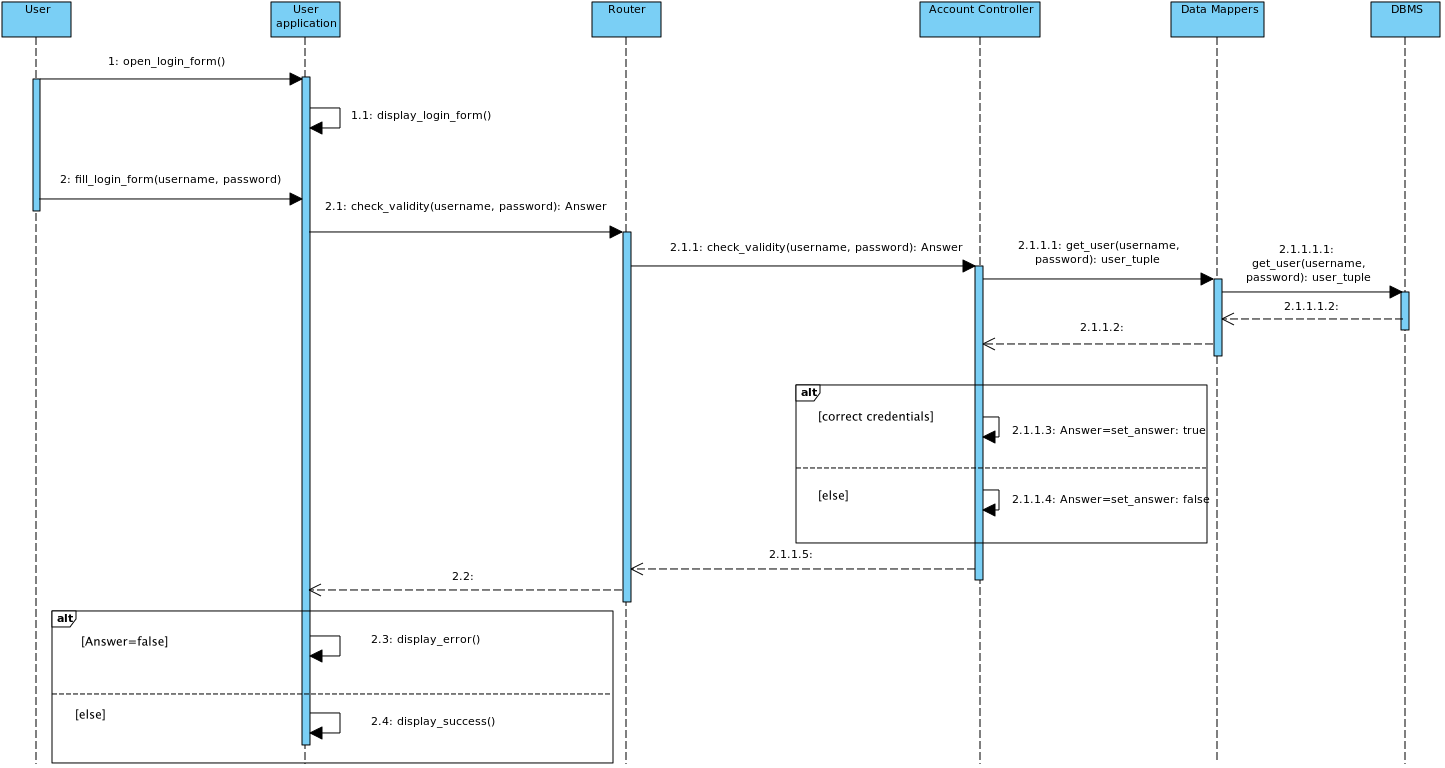
\includegraphics[scale=0.37, angle=-90, origin=c]{loginRuntimeView.png}
    \caption{User Login}
    \label{fig:loginRuntime}
\end{figure}

\subsubsection{Create Health Data}

\begin{figure}[H]
    \centering
    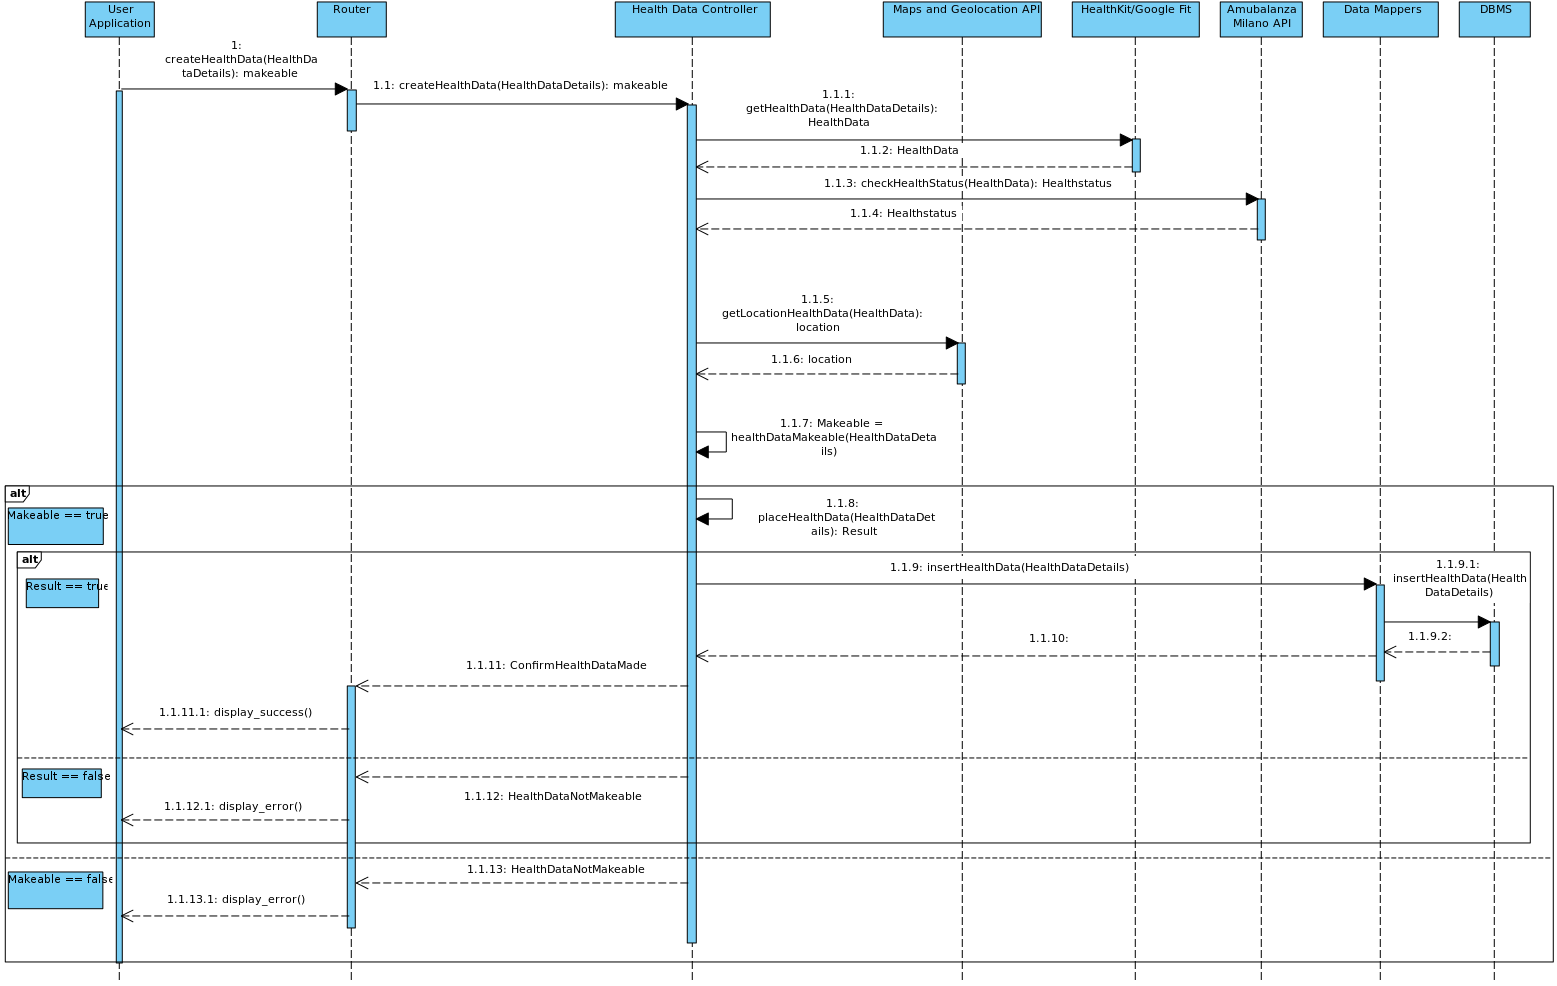
\includegraphics[scale=0.35, angle=-90, origin=c]{createHealthData.png}
    \caption{Health Data created for User.}
    \label{fig:createHealthData}
\end{figure}


\subsubsection{Create Run}

\begin{figure}[H]
    \centering
    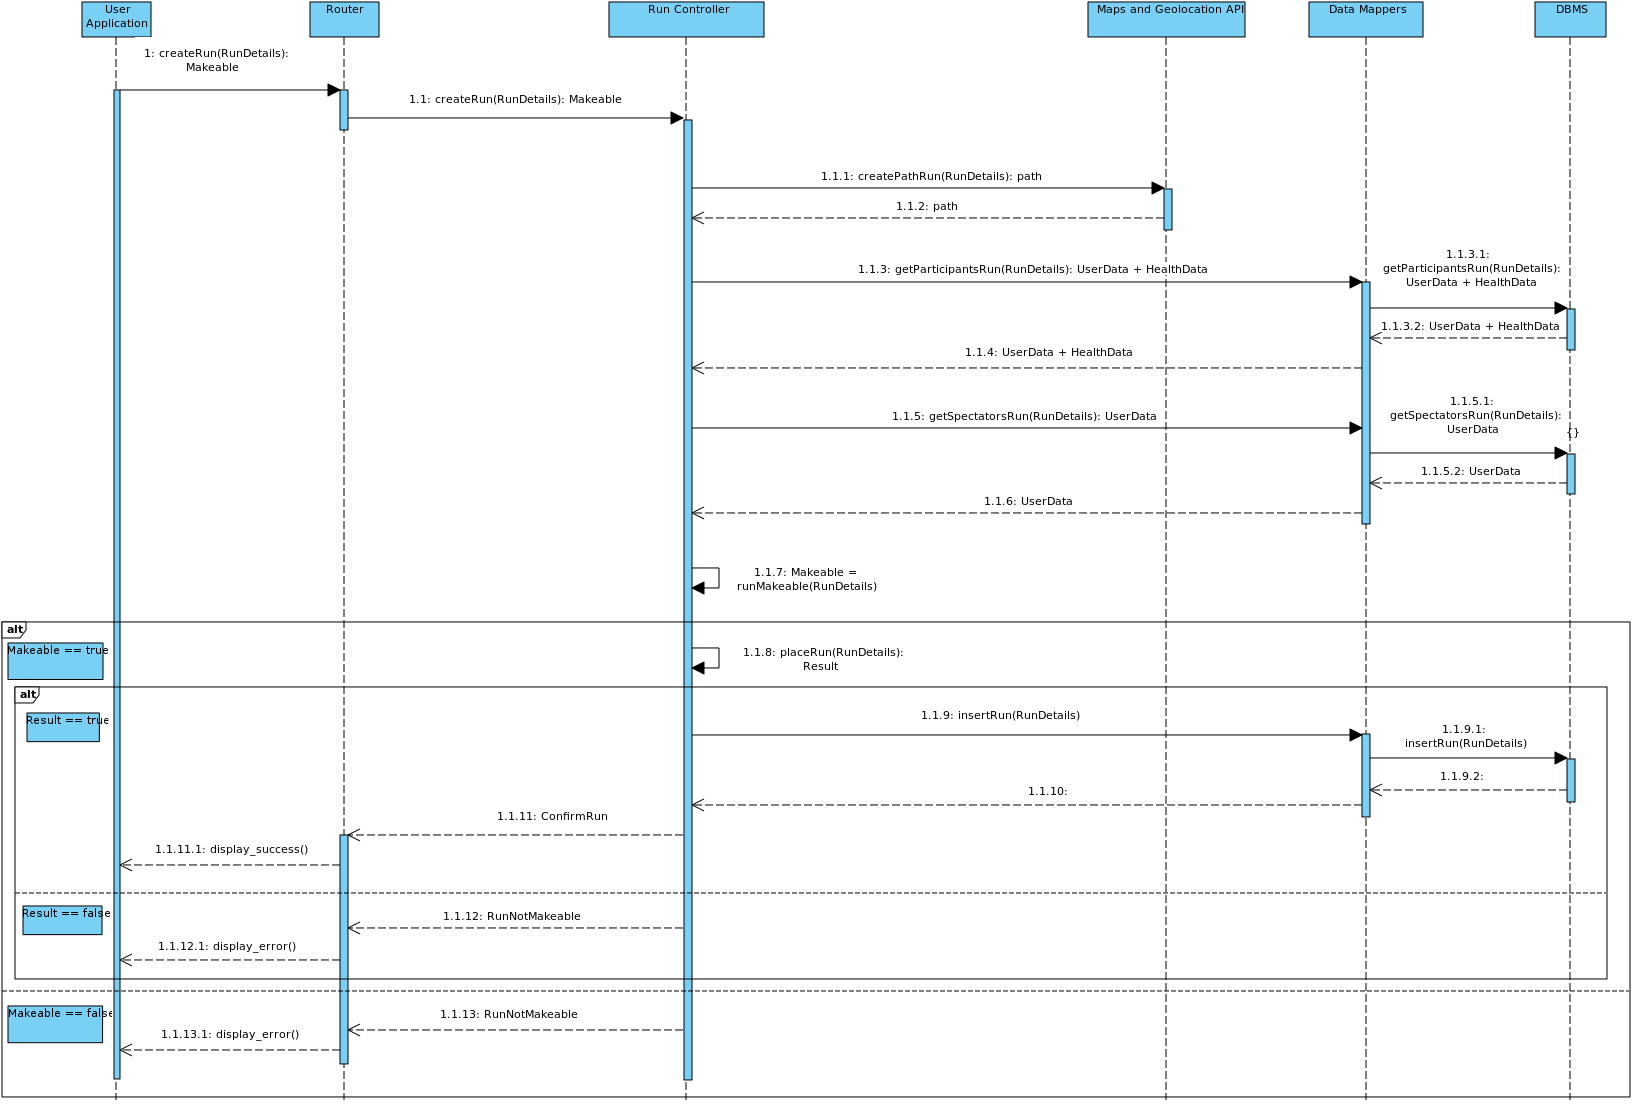
\includegraphics[scale=0.33, angle=-90, origin=c]{createRun.png}
    \caption{Run created by User.}
    \label{fig:createRun}
\end{figure}

\subsection{Component interfaces} 
In this section the interfaces through wich the different system's components interact will be described, and so will will the main methods associated with each interface.

\begin{itemize}
    \item The \textbf{UserAppIntferface} interface represents the way components can interact with the Server, being this the only interface through wich these two can communicate. This interface provides all of the methods provided by the \textbf{HealthDataIntferace} and the \textbf{RunIntferface}
    \item The \textbf{RunIntferface} interface represents the way components can interact with the Run Controller, responsible for managing all of the aspects associated with the run management. This interface provides the following methods: 
    \begin{enumerate}
        \item createRun(string: name, string: description, date: start, location: from, location: to ): receives the necessary information to create a run and creates it. 
        \item searchRun(date: start, location: from, location: to): receives parameters to search if there is a run that satisfies those requirements and returs runId if it is matched.
        \item deleteRun(int: runId): deletes the run with the specified Id. 
        \item enrollRun(int: runId, string: username): add the user to the runners of the specified run.
        \item spectateRun(int: runId): returns list of participants and some useful information about them. 
    \end{enumerate}
    
    \item The \textbf{AccountInterface} represents the way components interact with the Account Controller, responsible for managing all the aspects associated with the user account. This interface provides the following methods: 
    \begin{enumerate}
        \item createAccount(string: username, sting: email, string: password, boolean: individual, boolean: thirdPart): register a visitor into the system, creating an account for him distinguishing if it is a third part or an individual. 
        \item loginUser(string: username, string: password): logs a user into the system. 
        \item recoverPassword(string: user, string: email) sends a new password to user email, deleting the previous one. 
    \end{enumerate}
    \newpage 
    \item The \textbf{HealthDataInterface} represents the way components interact with the Health Data Controller, responsible for managing the aspects associated with the data accesses policies described previously. This interface provides the following methods: \begin{enumerate}
        \item getData(string: username): import all health data available from a certain user and save them in the system.
        \item requestData(string: username): send a request to a user in order to make its data available for another user. 
        \item acceptRequest(requestId, string: usernameAccept, string: usernameRequest) sends all the data from a user that accepted request to the user that requested them. 
        \item getDataGroup(): sends all the anonimized data of a group of individuals to a user that requested. 
        \item checkData(string: username) priodically checks health data of a certain user in order to understand if it is in danger.
    \end{enumerate}
    
    \item  The \textbf{DataAccessInterface} represent the way components can interact with the Data Mappers Component. It provides all the needed method and mechanisms to abstract the interaction between database and the system. 
    \item The \textbf{Maps and Geolocation API} interface represents the way components can interact with Maps and Geolocation service. It provides all the needed methods to get information about users location and the rutes for run. 
    \item The \textbf{Ambulanza Milano API} interface represents the way components interact with the emergency service of the city of Milan. It provides all the needed methods in order to allert an ambulance when a user is in danger and to give the position of the person to help. 
\end{itemize}


\subsection{Selected architectural styles and patterns}
\subsubsection{Client/Server Architecture} 
This application is made for run in devices that have limits regarding memory, computational power and battery as smartphones and smartwatches. So we choose this architectural style in order to keep all the logic of the program, wich is computationally quite heavy, on the server side, while the end-user only need to offer a simple ammount of presentation and sharing data functionality, avoiding it to use a big ammount of memory and pcu. This allows the system to be centralized, improving: 
\begin{itemize}
    \item Performance: system's files are only accessed by the server, and then sent to the users, so they are always in the same place, becoming easier to manage and faster to acces.
    \item Security: facilitates the implementation of security layers and protocols between the client and the server, setting up access rights to reach server for example. 
    \item Scalability: it is easy to change the logic of the server without any change on the client side.  
\end{itemize}


\section{Algorithm design}


\section{User Interface design}


\section{Requirements traceability}


\section{Implementation, integration and test plan}



\section{Effort spent}

\subsection{Michiel Janssen}

\begin{center}
\begin{tabular}{ |p{0.25\textwidth}|p{0.4\textwidth}|p{0.25\textwidth}| } 
 \hline
 \textbf{DATE} & \textbf{TASK} & \textbf{HOURS} \\ 
 \hline 
  28/11/2018 & Purpose, Scope, Definitions, Acronyms, Abbreviations & 2,5\\
  \hline
  29/11/2018 & High-level Components Description, Component View & 6\\
  \hline
  30/11/2018 & Database detailed analysis, Deployment View, Runtime View & 6,5\\
  \hline
  01/12/2018 & Server detailed analysis, Deployment View, Runtime View & 2\\
  \hline
  \textbf{TOTAL} & \multicolumn{2}{c|}{} \\ 
  \hline
\end{tabular}
\end{center}


\subsection{Erbol Kasenov}

\begin{center}
\begin{tabular}{ |p{0.25\textwidth}|p{0.4\textwidth}|p{0.25\textwidth}| } 
 \hline
 \textbf{DATE} & \textbf{TASK} & \textbf{HOURS} \\ 
  \hline
  18/11/2018 & Timetable, Purpose, Scope, Definitions, Acronyms, 
  Abbreviations, References document, Document Structure & 4.5\\ 
  
  \hline
  \textbf{TOTAL} & \multicolumn{2}{c|}{} \\ 
  \hline
\end{tabular}
\end{center}

\subsection{Lorenzo Casalini}

\begin{center}
\begin{tabular}{ |p{0.25\textwidth}|p{0.4\textwidth}|p{0.25\textwidth}| } 
 \hline
 \textbf{DATE} & \textbf{TASK} & \textbf{HOURS} \\ 
  \hline
 01/12/2018 & Component Interface, Architectural style & 3.5\\
  
  \hline
  \textbf{TOTAL} & \multicolumn{2}{c|}{} \\ 
  \hline
\end{tabular}
\end{center}







\end{document}
